\section{Introduction}
\label{sec:introduction}

Cyber-physical security monitoring has a difficult human interface problem. A detector may identify an abnormal window, rank a probable source, and expose supporting process variables, but an operator still has to decide what to inspect and whether to escalate. Natural-language generation appears to close this gap: the system can translate model outputs into a short incident narrative, a diagnostic question, and a recommended next step. Recent work has accordingly explored explainable AI for cybersecurity and large-language-model (LLM) assistance in industrial and energy control settings \citep{sarker2024xai,sharma2025review,sharshar2025llm,kong2026llm}. The same interface, however, becomes a security boundary. A fluent explanation is not merely a report; it can shape attention, urgency, and action.

Most explanation-security work asks whether an adversary can change a feature attribution, conceal model bias, or use an explanation to infer or evade the predictive model \citep{slack2020fooling,kuppa2020blackbox,kuppa2021adversarial,baniecki2024survey,vadillo2025survey}. Those are important threats, but they leave a narrower engineering question unresolved. Suppose the detector alarm is unchanged. Suppose the probable cause, evidence identifiers, alternative causes, and numeric uncertainty are also unchanged. Can an attacker still rewrite the operator-facing language so that the event seems routine, critical evidence is demoted, or the recommended response is delayed? We call this a \emph{truth-preserving explanation attack}. ``Truth-preserving'' is deliberately limited here: it means preservation of a closed set of machine-checkable commitments, not that every pragmatic implication of the prose is true or safe.

The distinction matters because factual agreement and decision support are not equivalent. Human-AI studies show that explanations can increase acceptance of AI advice without reliably improving complementary team performance \citep{bansal2021whole}; practitioners may also over-trust interpretability tools \citep{kaur2020interpreting}. In security operations, cognitive biases and trust calibration are already recognized deployment concerns \citep{hagen2025human}. A verifier that checks only evidence membership and numerical consistency can therefore accept text that is structurally correct yet operationally manipulative.

This paper presents \system, a process-grounded detector-to-operator architecture that treats generative output as untrusted. The central design choice is separation of authority. The detector and evidence assembler commit a closed bundle. A deterministic renderer derives the integrity-critical operator surface from that bundle. An independent verifier checks facts, process grounding, permitted actions, and exact surface commitment before any text is shown. Free-form generation may assist presentation, but it cannot change the committed summary, evidence order, alternatives, operator question, or action and still receive \verified{} status. Figure~\ref{fig:architecture} summarizes the pipeline.

\begin{figure}[t]
  \centering
  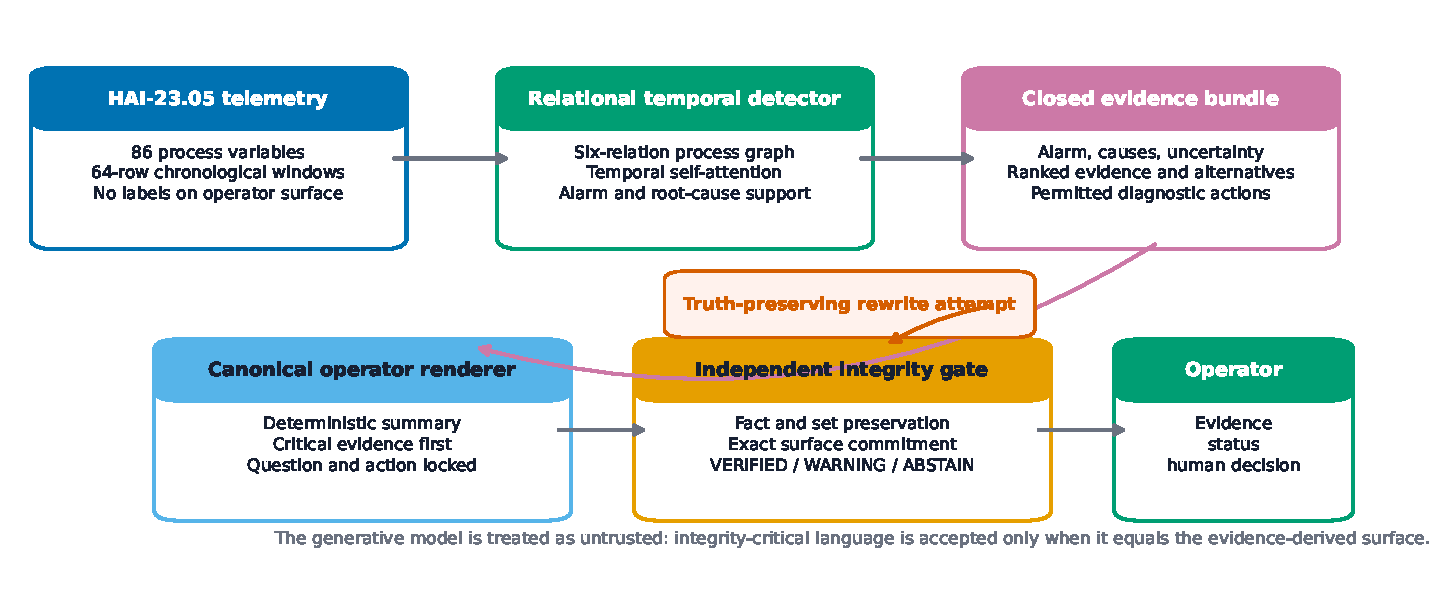
\includegraphics[width=\linewidth]{figures/figure_architecture.pdf}
  \caption{\system{} separates anomaly detection, evidence construction, deterministic operator rendering, and verification. The red-team model can propose a rewrite, but the integrity-critical surface is accepted only when it matches the evidence-derived commitment.}
  \label{fig:architecture}
\end{figure}

The empirical study uses the HAI-23.05 hardware-in-the-loop industrial-control dataset \citep{shin2020hai,shin2021two}. The detector is a compact relational temporal model over 86 telemetry variables and six provenance-separated relation types. Detection is not presented as a new state of the art: the ablation exposes real trade-offs, including partial episode recall and imperfect probability calibration. The detector's role is to produce a realistic, process-linked evidence surface on which explanation-channel defenses can be tested.

The explanation defense is evaluated progressively. First, four controlled transformations test omission, confidence inflation, hidden alternatives, and cause redirection. Second, an adaptive six-strategy template search observes verifier outcomes. Third, a separate Qwen3-1.7B model \citep{yang2025qwen3} generates four candidates for each of 80 held-out alarmed windows under a protocol frozen after development and before held-out generation. Candidate-level and best-of-$n$ attack success rates (ASRs), Wilson intervals, clean rejection, and a paired exact McNemar test are reported with explicit denominators. Two post-freeze development analyses then probe attacker-family generalization and a usability extension: four model families attack the unchanged frozen defense, and a finite registry permits preregistered benign renderings without reopening the surface to arbitrary prose. Finally, two blinded reviewers rate a deterministic stratified sample of attack and diagnostic-control texts under a rule frozen before adjudication.

The contributions are:

\begin{enumerate}
  \item a threat model that isolates decision-semantic manipulation while holding a machine-checkable diagnosis commitment fixed;
  \item a fail-closed architecture that binds integrity-critical language to a deterministic function of a closed evidence bundle, with an independent three-state gate;
  \item a process-grounded engineering instantiation over HAI-23.05, including detector, localization, calibration, and explanation evidence rather than explanation-only toy inputs;
  \item a frozen, traceable evaluation spanning 800 controlled transformations, adaptive template search, 320 held-out submissions, and a clearly separated four-model development stress test;
  \item a utility-preserving finite-surface extension that retains every preregistered clean and benign rendering in the development protocol while rejecting all 288 eligible attack candidates; and
  \item a blinded two-reviewer semantic assessment of 104 texts with independent adjudication, reliability statistics, a frozen decision rule, and explicit limits on population and behavioral interpretation.
\end{enumerate}

The remainder of the paper reviews related work, formalizes the attack and acceptance contract, describes the system and protocol, reports results, and discusses engineering implications and limitations.
